%*****************************************
\chapter{The $\lambda$-calculus}\label{ch:lambda}
%*****************************************
\section{History and overview}
$\lambda$-calculus has attracted from its birth in the thirties some of the best minds of the century. Its elegance and simplicity, together with its power have fascinated thousands of people in Logic, Computer Science, Math and Philosophy. A detailed historical survey is \cite{cardone_lambda-calculus_2009}.
\subsection{The Birth of Computer Science}
Alonzo Church invented the $\lambda$-calculus with the aim of providing a
foundation for logic which would be more natural than Russell’s type theory or
Zermelo’s set theory \cite{church_set_1932}. Church's system was a type-free logic with
unrestricted quantification but without the law of excluded middle. However very soon his system was proved inconsistent by Kleene and Rosser \cite{kleene_inconsistency_1935}. Abandoned the foundational aspects, the system restricted to the functional part, i.e. without logic, turned out to be very interesting. It allowed the very first proof of non-decidability of a problem (the convertibility problem) \cite{church_unsolvable_1936} and soon after the negative answer to the \textit{Entscheidungsproblem} \cite{church_note_1936}. After the proofs of equivalence between the $\lambda$-calculus and Turing machines \cite{turing_computability_1937}, and between the $\lambda$-calculus and the partial recursive functions \cite{kleene_$lambda$-definability_1936}, Church's Thesis could be stated: $\lambda$-definability captures the intuitive notion of effective calculability.
\subsection{Functions as Rules}
In $\lambda$-calculus, unlike set theory, functions are first-class citizens. Moreover, unlike set theory, functions are defined intentionally, i.e. through the rule that allows to pass from the argument to the result. This way computing a function becomes a rewriting process. $\lambda$-notation serves to this goal. Computing a function means to substitute the argument in the body where there are occurrences of the binded variable. In a $\lambda$-calculus extended with the $+$ operator and natural numbers one could write the following:
$$
\lambda x. x+x+x
$$
that is a function that takes an argument $x$ and returns as result $x+x+x$. Functions are applied to arguments, for example:
$$
(\lambda x. x+x+x)3\red3+3+3\red 9.
$$
$\lambda$-abstraction binds a single variable. However we are interested in writing functions like $x+y$ which have more than one argument. Frege in \cite{frege_basic_1893} and then Schönfinkel (the father of Combinatory Logic) in \cite{schonfinkel_uber_1924} proposed a method, now called curryfication, to overcome this problem. The trick consists in the partial application of a function.  We illustrate it with an example. If we want to compute $x+y$ on two arguments, say $a$ and $b$, first we compute a one-argument function that sums $a$ to its argument and then we apply it to $b$.
$$
((\lambda x.(\lambda y.x+y))a)b\red(\lambda y.a+y)b\red a+b.
$$
This is possible in the $\lambda$-calculus because functions can return other functions (and taking functions as parameters). That means that the $\lambda$-calculus is a higher-order formalism.
\subsection{A Programming Languages Foundation}
The main difference between high level programming languages and low level ones is that the former are machine independent. For this reason models of high level languages should be machine-independent too. Turing machines, for example, are not suitable to describe many of the main mechanisms of programming languages, such as function calls or type systems. $\lambda$-calculus turns out to be very useful in this sense. In fact, already in the sixties, a translation between Algol 60 and the $\lambda$-calculus was given \cite{landin_correspondence_1965-1, landin_correspondence_1965}. This way, $\lambda$-calculus provided a formal semantics to a real programming language, Algol 60, the ancestor of languages such as \texttt{C} or \texttt{Pascal}. Moreover, Landin proposed an abstract machine, called \texttt{SECD} (Stack, Environment, Control, Dump) \cite{landin_mechanical_1964}, specifically devised to evaluate expressions of the $\lambda$-calculus. This seminal work opened the field of the formal study of operational semantics of programming languages, culminated with the fundamental work of Gordon Plotkin \cite{plotkin_call-by-name_1975}, which in fact used the \texttt{SECD} machine and \texttt{ISWIM}, a sugared $\lambda$-calculus proposed by Landin \cite{landin_next_1966} as a paradigmatic programming language. Concepts like call-by-name and call-by-value were indeed formalised through the use of the $\lambda$-calculus and modern functional programming languages like \texttt{Haskell} or the \texttt{ML} family were directly inspired by \texttt{ISWIM}. On the other hand, typed $\lambda$-calculi directly inspired typed programming languages. For example the Hindley-Milner type system \cite{hindley_principal_1969,milner_theory_1978}, originally devised for the $\lambda$-calculus, is the core of the type systems adopted in \texttt{Haskell} and \texttt{ML}. Moreover, the $\lambda$-calculus was the driver for the study of effetctful languages. Mechanisms to introduce impurities, such as input/output or exception handling, in pure functional languages like \texttt{Haskell} were first introduced in the abstract setting of the $\lambda$-calculus. Monads \cite{moggi_notions_1991} are the most notable example.
\section{The Syntax}
We now define a specific ARS, the $\lambda$-calculus. We start defining the set of its terms. As usual in theoretical computer science terms are inductively defined by a context-free grammar \cite{backus_syntax_1959}.
\begin{definition}
	Assume a countable infinite set $\mathcal{V}$ of variables. The
	$\lambda$-\emph{calculus} is the language of terms defined by
	the following grammar:
	$$
	\termone,\termtwo\bnf\varone\in\mathcal{V}\midd\termone\termtwo\midd\abstr{\varone}{\termone}
	$$
	We denote by $\Lambda$ the set of all $\lambda$-terms.
\end{definition}
Since $\lambda$-terms are defined inductively from other $\lambda$-terms via application and abstraction, it is natural to define a function that maps each term to the set of its subterms. We will often use a pattern-matching-like syntax to define properties of $\lambda$-terms. In this case the match is against the rule of the grammar used to form the term (akin to sum types in functional programming languages).
\begin{THESIS}
	\begin{definition}
		The set of \emph{subterms} $\mathsf{Sub(\mathit{\termone})}$ of a term $\termone$ is defined inductively on the structure of $\termone$ as follows.
		\begin{align*}
		&\mathsf{Sub}(x)=\{x\},\\
		&\mathsf{Sub}(\termtwo\termthree)=\mathsf{Sub}(\termtwo)\cup \mathsf{Sub}(\termthree)\cup\{\termtwo\termthree\},\\
		&\mathsf{Sub}(\lambda x.\termtwo)=\mathsf{Sub}(\termtwo)\cup \{\lambda x.\termtwo\}.
		\end{align*}
	\end{definition}
\end{THESIS}
\begin{THESIS}
	The concept of bound and free variables is ubiquitous in logic. Informally, names of bounded occurrences of variables are meaningless, in the sense that they can be renamed without changing the semantics of a term, provided that new names are \emph{fresh}, i.e. they do not occur anywhere in the term. This observation leads to the definition of $\alpha$-conversion.
	\begin{definition}
		A variable $x$ occurs \emph{bound} in $\termone$, if $\lambda x.\termtwo\in\mathsf{Sub(\mathit{\termone})}$ for some term $\termtwo$. The set of \emph{free variables} $FV(\termone)$ of a term $\termone$ is defined inductively on the structure of $\termone$ as follows.
		\begin{align*}
		&FV(x)=\{x\},\\
		&FV(\termtwo\termthree)=FV(\termtwo)\cup FV(\termthree),\\
		&FV(\lambda x.\termtwo)=FV(\termtwo)\setminus\{x\}.
		\end{align*}
	\end{definition}
	\begin{definition}
		Two terms $\termone$ and $\termtwo$ are said to be \emph{$\alpha$-convertible} if one can derive the same term from both purely by renaming bound occurrences of variables to fresh variables.
	\end{definition}
	Since $\alpha$-conversion is an equivalence relation, from now on we consider $\lambda$-terms modulo $\alpha$-equivalence. Indeed if two terms $\termone$ and $\termtwo$ are $\alpha$-convertible we consider them equivalent at syntactic level and we write $\termone\equiv\termtwo$. Moreover it is worth mentioning that there exist different representations of $\lambda$-terms in which there are not bound variables at all. The most famous is the use of De Brujin indexes, used in most compilers and interpreters of functional programming languages \cite{de_bruijn_lambda_1972}.
	
\end{THESIS}
\begin{THESIS}
	In order to define $\beta$-reduction, the reduction relation of the $\lambda$-calculus, we need to formally define the concept of substitution. 
	We assume from now on the \emph{Barendregt's variable convention} for which every term has all bound variables \emph{distinct} from each other and from any free variable. This can be done since we are considering terms modulo $\alpha$-equivalence.
	\begin{definition}
		We denote by $\termone\{\termtwo/x\}$ the \emph{(capture-avoiding) substitution} of variable $x$ by term $\termtwo$ in term $\termone$ performed in the following way.
		\begin{align*}
		&x\{\termtwo/x\}=\termtwo,\\
		&y\{\termtwo/x\}=y\qquad\textrm{if $x\not\equiv y$},\\
		&(\termone\termthree)\{\termtwo/x\}=(\termone\{\termtwo/x\}\termthree\{\termtwo/x\}),\\
		&(\lambda y.\termone)\{\termtwo/x\}=(\lambda y.\termone\{\termtwo/x\})\qquad\textrm{if $x\not\equiv y$ and $y\not\in FV(\termtwo)$},\\
		&(\lambda y.\termone)\{\termtwo/x\}=\lambda z.\termone\{z/y\}\{\termtwo/x\}\quad\textrm{if $x\equiv y$ or $y\in FV(\termtwo)$}.
		\end{align*}
		where $z$ is a fresh variable, i.e. it does not occur in $\termone$ or $\termtwo$.
	\end{definition}
	The following Lemma asserts formally commutativity of substitutions.
	\begin{lemma}[Substitution Lemma]
		For any $\termone,\termtwo,\termthree\in\Lambda$ if $x\neq y$ and $x\not\in FV(\termthree)$, then
		$$
		\termone\{\termtwo/x\}\{\termthree/y\}\equiv\termone\{\termthree/y\}\{\termtwo\{\termthree/y\}/x\}.
		$$
	\end{lemma}
\end{THESIS}
Reduction will be defined based on the notion of a context, which
needs to be given a formal status.
\begin{definition}
	We define (one-hole) \emph{contexts} by the following grammar:
	$$
	\contone,\conttwo\bnf\Box\midd\contone\termone\midd\termone\contone\midd\abstr{\varone}{\contone}
	$$
	We denote with $\Lambda_\Box$ the set of all contexts.
\end{definition}
Intuitively, contexts are $\lambda$-terms with a hole that can be
filled with another $\lambda$-term. We indicate with
$\contone[\termone]$ the term obtained by replacing $\Box$ with
$\termone$ in $\contone$. Those $\lambda$-terms in the form
$\rdxone=(\lambda x.\termone)\termtwo$ are called \emph{$\beta$-reducible expressions} or
$\beta$-\emph{redexes} and $\termone\{\termtwo/x\}$ is said to be
the \emph{contractum} of $\rdxone$. This is justified by the following definition.
\begin{definition}
	The relation of $\beta$-\emph{reduction}, $\redbeta\subseteq\Lambda\times\Lambda$, is defined as the contextual clojure of the $\beta$-rule
	$$
	(\lambda x.\termone)\termtwo\rightarrow_\beta\termone\{\termtwo/x\}
	$$
	i.e.
	$$
	\redbeta = \{(\contone[(\lambda x.\termone)\termtwo],\, \contone[\termone\{\termtwo/x\}])\, |\, \termone, \termtwo\in\Lambda, \contone\in\Lambda_\Box\}.
	$$
\end{definition}
This way we have defined the $\lambda$-calculus as the ARS $(\Lambda,\redbeta)$. We denote by $\Lambda_\mathsf{WN}$ the set of weakly normalising terms of $\Lambda$. In the following sections a restriction of the $\beta$-reduction will be useful.
\begin{definition}
	The relation of $\mathsf{ANF}$-$\beta$-\emph{reduction}, $\redbetaanf\subseteq\Lambda\times\Lambda$, is defined as
	$$
	\redbetaanf = \{(\contone[(\lambda x.\termone)\termtwo],\, \contone[\termone\{\termtwo/x\}])\, |\, \termone, \termtwo\in\Lambda,\,\termtwo\in\textbf{NF}(\Lambda),\, \contone\in\Lambda_\Box\}.
	$$
\end{definition}
This restriction allows to contract a redex only if its argument is already in normal form. In some way resembles the call-by-value evaluation order, in which arguments have to be evaluated before being passed to a function.
\begin{definition}
	We call \emph{$\beta$-equivalence} the equivalence closure of the $\beta$-reduction relation, and we write $\termone=_\beta\termtwo$ if $\termone$ is $\beta$-equal to $\termtwo$.
\end{definition}
The congruence $=_\beta$ generated by $\beta$-reduction has the intuitive meaning ``two terms are $\beta$-equal if and only if they are the \emph{same} program''. Sometimes this is too strict. If we want to consider equal two terms when they return the same results on the same arguments, we have to add a new axiom, called the $\eta$-rule. This way a new equational theory $=_{\beta\eta}$ is generated.
\begin{definition}
	Two $\lambda$-terms $\termone$ and $\termtwo$ are \emph{extensionally equal} if for each $\lambda$-term $\termthree$, $\termone\termthree=_{\beta\eta}\termtwo\termthree$. This is equivalent to the addition of the following rule:
	$$
	\lambda x.\termone x=_\eta\termone \qquad\textrm{if }x\not\in FV(\termone).
	$$
\end{definition}
This latter formulation highlights that $\eta$-rule is not derivable from $\beta$-rule. In fact $\lambda x.yx=_\eta y$ while $\lambda x.yx\not=_\beta y$, since they are different normal forms.
\subsection{Two Subcalculi of $\Lambda$}
%%%%%%%%%%%%%%%%%%%%%%%%%%%%%%%%%%%%%%%%
Full $\lambda$-calculus is very powerful and flexible but it has a complicated dynamics. Sometimes it is useful to restrict ourselves to a subset of terms. In particular we focus our attention on two subsystems where terms satisfy a predicate on the number of occurrences of free variables. These systems are meaningful because they are \emph{stable} w.r.t. $\beta$-reduction i.e. if $\termone\in S$ and $\termone\redbeta\termtwo$ then $\termtwo\in S$. A comprehensive treatment is in \cite{sinot_sub-lambda-calculi_2008}.
%%%%%%%%%%%%%%%%%%%%%%%%%%%%%%%%%%%%%
\subsubsection{The $\lambda I$-calculus.}
%%%%%%%%%%%%%%%%%%%%%%%%%%%%%%%%%%%%%
The $\lambda I$-calculus was the original calculus studied by Alonzo
Church in the '30 \cite{church_unsolvable_1936}, while
\cite{barendregt_lambda_1984} contains a whole section dedicated to
it. In $\lambda I$-calculus there is no \emph{cancellation}, in that
variables have to occur free \emph{at least once} when forming
abstractions. Terms of the $\lambda I$-calculus are not strongly
normalising in general. As an example, $\bm{\Omega}$ is a $\lambda I$-term.
One can prove, however, the following important result.
\begin{theorem}
	For each term $\termone\in\Lambda_I$, if $\termone$ is weakly normalising, then it is strongly normalising.
\end{theorem}
In other words, all strategies are qualitatively equivalent. This does \emph{not} mean, however, that they are quantitatively equivalent. A consequece of this fact is that the ARS $(\Lambda_I,\redbeta)$ does not satisfy the weak diamond property, as witnessed by the following example.
\begin{example}
	Let $\bm{I}=\lambda x.x$ and $\termone=(\lambda x.xx)(\bm{II})$. Two reducts of $\termone$ are $\termtwo=(\bm{II})(\bm{II})$ and $\termthree=(\lambda x.xx)\bm{I}$. Clearly it does not exist a term $\termfour$ such that $\termtwo\redbeta\termfour$ and $\termthree\redbeta\termfour$. In fact $\termthree\redbeta\bm{II}$, while $\termtwo\redbeta(\bm{II})\bm{I}$ or $\termtwo\redbeta\bm{I}(\bm{II})$. The reduction process is sketched in Figure~\ref{figure:couterexample}.
\end{example}
\begin{figure}
	\fbox{
		\begin{minipage}{.96\textwidth}
	\begin{center}
		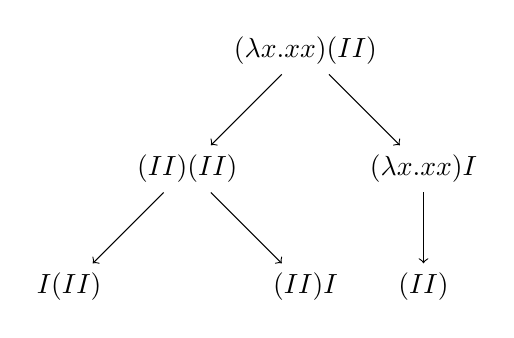
\begin{tikzpicture}
		[node distance=20mm, auto, transform shape]
		\node (m) at (0,0) {$(\lambda x.xx)(\bm{II})$};
		\node (n) at (-1.5,-1.5) {$(\bm{II})(\bm{II})$};
		\node (l) at (1.5,-1.5) {$(\lambda x.xx)\bm{I}$};
		\node (p) at (0,-3) {$(\bm{II})\bm{I}$};
		\node (q) at (-3,-3) {$\bm{I}(\bm{II})$};
		\node (r) at (1.5,-3) {$(\bm{II})$};
		\draw (m) edge[->] node[left=5pt] {} (n);
		\draw (m) edge[->] node[right=5pt] {} (l);
		\draw (n) edge[->] node[left=5pt] {} (p);
		\draw (n) edge[->] node[right=5pt] {} (q);
		\draw (l) edge[->] node[right=5pt] {} (r);
		\end{tikzpicture}
	\end{center}
\end{minipage}}
	\caption{All possible reduction sequences of length 2 of the term $\termone=(\lambda x.xx)(\bm{II})$. No one forms a diamond.}
	\label{figure:couterexample}
\end{figure}
%%%%%%%%%%%%%%%%%%%%%%%%%%%%%%%%%%%%%
\subsubsection{The $\lambda A$-calculus.}
%%%%%%%%%%%%%%%%%%%%%%%%%%%%%%%%%%%%%
The $\lambda A$-calculus is the dual of $\lambda I$-calculus and it is
sometimes called \emph{affine} $\lambda$-calculus in the
literature. It is a very weak calculus in which variables bound by
abstractions occur \emph{at most once} free in the abstraction's body,
thus forbidding \emph{duplication}. The $\lambda A$-calculus is strongly
normalising, in a very strong sense: every reduction sequence from a term
$\termone$ has length bounded by the size of $\termone$. This fact confirms that \emph{copy} is the source of complexity in the $\lambda$-calculus. Controlling copy structurally can indeed bound the length of computations, as shown by different works \cite{baillot_soft_2004,terui_light_2007} in the research area of Implicit Computational Complexity \cite{dal_lago_short_2012} via Linear Logic \cite{girard_linear_1987}.
\section{Fundamental Meta-Theory}
In this section we report some fundamental results in the meta-theory of the $\lambda$-calculus. From the variety of results developed in more than 80 years, we have chosen two seminal theorems, published in the mid-30s.
\subsection{Confluence}
Classical $\lambda$-calculus is deterministic, in that if a $\lambda$-term has a normal form, then it is unique, independently from the reduction path followed. As we have seen in the Section devoted to Abstract Rewriting, uniqueness of normal form is an easy corollary of confluence. The first proof of confluence is due to Church and Rosser \cite{church_properties_1936} in the early days of the $\lambda$-calculus, but many others appeared later. The standard proof of this result is due to Tait and Martin-Löf \cite[Section~3.2]{barendregt_lambda_1984}, based on the notion of parallel reduction. Barendregt in his monograph presents also three other proofs, one more direct \cite[Section~11.1]{barendregt_lambda_1984}, one based on the notion of development \cite[Section~11.2]{barendregt_lambda_1984} and one based on the labeled $\lambda$-calculus \cite[Section~14.2]{barendregt_lambda_1984} (originally presented in \cite{levy_reductions_1978}). Because of the importance of this result, the Tait-Martin-Löf proof was further simplified in \cite{takahashi_parallel_1995} and other subsequent works. Church-Rosser theorem was also object of interest for people interested in formalised mathematics and interactive theorem provers as witnessed by various papers containing different formalisations written for different theorem provers \cite{shankar_mechanical_1988,huet_residual_1994}.
\begin{theorem}[Church-Rosser]
	The relation $\redbeta$ on $\Lambda$ is confluent.
\end{theorem}
\begin{corollary}
	Let $\termone\in\Lambda$ be a $\lambda$-term. If $\termone\redbeta\termtwo$ and $\termone\redbeta\termthree$, where $\termtwo,\termthree\in\textbf{NF}(\Lambda)$, then $\termtwo\equiv\termthree$.
\end{corollary}
\subsection{Expressiveness}
The $\lambda$-calculus, as we have defined it, in the previous section, turns out to be a Turing-complete formalism. This means that we should be able to use it as a programming language. We are not going to discuss in detail all the encodings, we just limit to a few illuminating examples. For a complete treatment, the interested reader can refer to \cite{barendregt_lambda_1984}.
\paragraph{Integers}
Integer numbers can be encoded as $\lambda$ terms in the following way. They are named Church numerals because this was the original encoding provided by Church \cite{church_set_1933}. In particular, for each $n\geq 0$:
$$
\lceil n\rceil=\lambda f.\lambda x.(f^nx)
$$
where $f^nx$ is inductively defined by
$$
f^0x=x\,,\qquad f^kx=f(f^{k-1}x)\,.
$$
For example,
\begin{itemize}
	\item $\lceil zero\rceil=\lambda f.\lambda x.x$
	\item $\lceil one\rceil=\lambda f.\lambda x.(fx)$
	\item $\lceil two\rceil=\lambda f.\lambda x.(f(fx))$
\end{itemize}
\paragraph{Arithmetics}
Once defined numerals, one wants to use them. We give here combinators for addition, multiplication and exponentiation:
\begin{itemize}
	\item $\mathbf{A}=\lambda x.\lambda y.\lambda p.\lambda q.(xp(ypq))$,
	\item $\mathbf{M}=\lambda x.\lambda y.\lambda z.(x(yz))$,
	\item $\mathbf{E}=\lambda x.\lambda y.yx$.
\end{itemize}
\begin{proposition}
	$\mathbf{A}$, $\mathbf{M}$ and $\mathbf{E}$ perform, respectively, addition, multiplication and exponentiation when applied to Church numerals, i.e.
	\begin{itemize}
		\item $\mathbf{A}\lceil n\rceil\lceil m\rceil\redbetared{}\lceil n+m\rceil$,
		\item $\mathbf{M}\lceil n\rceil\lceil m\rceil\redbetared{}\lceil n*m\rceil$,
		\item $\mathbf{E}\lceil n\rceil\lceil m\rceil\redbetared{}\lceil n^m\rceil$, except for $m=0$.
	\end{itemize}
\end{proposition}
The reader can note how easy the whole process is w.r.t other Turing-complete formalisms, such as Turing machines. Sketching a single-tape Turing machine performing multiplication would not be in fact an easy task at all.
\paragraph{$\lambda$-definability}
Besides basic arithmetical operations one could show how to encode in the $\lambda$-calculus all partial recursive functions. 
\begin{definition}
	A partial function $f:\mathbb{N}^m\rightarrow\mathbb{N}$ is \emph{$\lambda$-definable} if there exists a $\lambda$-term $\mathbf{F}$ such that for each $n_1\cdots n_m\in\mathbb{N}$,
	\begin{enumerate}
		\item If $f(n_1\cdots n_m)=n$, then $\mathbf{F}\lceil n_1\rceil\cdots\lceil n_m\rceil\twoheadrightarrow \lceil n\rceil$.
		\item If $f(n_1\cdots n_m)$ is undefined, then $\mathbf{F}$  has no normal form.
	\end{enumerate}
\end{definition}
Since one can prove that it is possible to encode in the $\lambda$-calculus the so-called initial functions, together with composition, projection, minimisation and primitive recursion operators, the $\lambda$-calculus is a Turing-complete language, characterising our intuitive notion of computability.
\begin{theorem}
	A function is $\lambda$-definable if and only if it is partial recursive.
\end{theorem}
Actually, one does not need full $\lambda$-calculus to have a Turing-complete language, because also the $\lambda I$-calculus has the same characteristic. In this framework Church gave the first example of a recursively enumerable set which is not recursive.
\begin{theorem}
	The set $\{\termone\in\Lambda\,|\,\termone\textrm{ has normal form}\}$ is recursively enumerable, but not recursive.
\end{theorem}
\section{Strategies}
We have already defined what a reduction strategy is, in the abstract. Now we are going to report some results regarding some concrete strategies for the $\lambda$-calculus. Typically, strategies are defined giving the position of the redex to be reduced. Different strategies can lead to completely different reduction sequences and thus to completely different computations. Some, for example, can be non-terminating, while others can terminate in just one step, though starting from the same term. Investigation of reduction strategies is an active field in the programming language community because of the great impact they have on performances. A we have already pointed out, one could ask if a minimal reduction strategy exists, and in that case if it is computable. With minimal we intend leading to normal form, if there is one, in the minimum number of $\beta$-steps.
\begin{proposition}[\cite{barendregt_notes_1976}]
	There exists a minimal strategy for the $\lambda$-calculus.
\end{proposition}
This is a trivial result. A less trivial one is the following.
\begin{theorem}[\cite{barendregt_notes_1976}]
	There exists no recursive minimal strategy for the $\lambda$-calculus.
\end{theorem}
This latter negative result can be strengthened in the following sense.
\begin{theorem}[\cite{kathail_optimal_1990}]
	For any $k>0$, there is no recursive reduction strategy that can reduce any $\lambda$-term to normal form (if any) in no more than $k\cdot m$ steps, where $m$ is the minimum number of $\beta$-steps needed to reduce the term.
\end{theorem}
Since there is no hope to devise strategies that are good in any context, we start defining two classical strategies and then reporting some results about them.
\begin{definition}
	\emph{Leftmost-outermost} $(\pslo)$ is a deterministic reduction
	strategy in which $\pslo(\termone)=\termtwo$ if and only if
	$\termone\redbeta\termtwo$ and the redex contracted in $\termone$ is
	the \emph{leftmost} among the ones in $\termone$ (measuring the
	position of a redex by its beginning). If $\pslo(\termone)=\termtwo$,
	we write $\termone\redlo\termtwo$.
\end{definition}
\begin{definition}
	\emph{Rightmost-innermost} $(\psri)$ is a deterministic reduction
	strategy in which $\psri(\termone)=\termtwo$ if and only if
	$\termone\redbeta\termtwo$ and the redex contracted in $\termone$ is
	the \emph{rightmost} among the ones in $\termone$ (measuring the
	position of a redex by its beginning). Again, if
	$\psri(\termone)=\termtwo$, we write $\termone\redri\termtwo$.
\end{definition}
\begin{example}\label{example:canc}
	Let $\bm{\omega}=\lambda x.xx$ and
	$\bm{\Omega}=\bm{\omega\omega}$. We now consider the reduction of
	the term $(\lambda x.y)\bm{\Omega}$ according to leftmost-outermost and
	rightmost-innermost stratgies.
	\begin{align*}
		(\lambda x.y)\bm{\Omega}&\redlo y\\
		(\lambda x.y)\bm{\Omega}&\redri(\lambda x.y)\bm{\Omega}\redri(\lambda x.y)\bm{\Omega}\redri\cdots
	\end{align*}
	The term $\bm{\Omega}$ is a looping combinator i.e. it reduces to
	itself. However, in $(\lambda x.y)\bm{\Omega}$ the argument
	$\bm{\Omega}$ is discarded since the function returns the constant
	$y$. Thus leftmost-outermost (akin to call-by-name in functional
	programming languages) yields a normal form in one step. Conversely,
	rightmost-innermost (akin to call-by-value) continues to evaluate
	the argument $(\lambda x.y)\bm{\Omega}$, though it is useless, and
	rewrites always the same term, yielding to a non-terminating
	process.
\end{example}
\begin{example}\label{example:copy}
	Let $\bm{I}=\lambda x.x$. We now consider the reduction of the term
	$(\lambda x.xx)(\bm{II})$, according to $\pslo$ and $\psri$
	strategies, as above.
	\begin{align*}
		(\lambda x.xx)(\bm{II})&\redlo (\bm{II})(\bm{II}) \redlo
		\bm{I}(\bm{II}) \redlo \bm{II} \redlo \bm{I}\\
		(\lambda x.xx)(\bm{II})&\redri (\lambda x.xx)\bm{I} \redri \bm{II} \redri \bm{I}
	\end{align*}
	Here the argument $\bm{II}$ is duplicated and thus it is much more convenient
	to reduce it before it is copied, as in
	rightmost-innermost. Leftmost-outermost does, indeed, some useless
	work.
\end{example}
\begin{THESIS}
	In the study of strategies, it is interesting to see what happens to all the redexes that are not reduced. After a reduction step, are they cancelled, are they duplicated? The concept of residual of a redex in a term formalises this idea.
	\begin{definition}[Residuals \cite{xi_upper_1999}]
		Let $\termone$ be a term and $\rdxone=(\lambda x.\termtwo)\termthree$ one of its redexes. If $\termone\redbetardx{\rdxone}\termfour$, then for each redex $\rdxtwo$ of $\termone$ the \emph{residuals} of $\rdxtwo$ are defined in the following way.
		\begin{itemize}
			\item $\rdxtwo$ is $\rdxone$. Then $\rdxtwo$ has no residuals in $\termfour$.
			\item $\rdxtwo$ is in $\termtwo$. Then $\rdxtwo\{\termthree/x\}$ in $\termtwo\{\termthree/x\}$ is the only residual of $\rdxtwo$ in $\termfour$.
			\item $\rdxtwo$ is in $\termthree$. All copies of $\rdxtwo$ in $\termtwo\{\termthree/x\}$ are residuals of $\rdxtwo$ in $\termfour$.
			\item $\rdxtwo$ contains $\rdxone$. Then the residual of $\rdxtwo$ is the term obtained by replacing $\rdxone$ in $\rdxtwo$ with $\termtwo\{\termthree/x\}$.
			\item Otherwise $\rdxtwo$ is not affected and is its own residual in $\termfour$.
		\end{itemize}
		The residual relation is transitive.
	\end{definition}
	\subsection{Standard Sequences and Leftmost Strategies}
	Through the concept of residual it is possible to define what a standard reduction sequence is. Standard reduction sequences are important because a fundamental theorem in the theory of the $\lambda$-calculus, the Standardisation Theorem, states that every reduction sequence can be standardised, yielding as a corollary that leftmost-outermost strategy is normalising. We show step-by-step how to derive this result, although omitting the proofs, that however can be found in the references.  
	\begin{definition}
		A reduction sequence $\sigma:\termone\redbetardx{\rdxone_1}\termone_1\redbetardx{\rdxone_2}\cdots\termone_n=\termtwo$ is \emph{standard} if for all $1\leq i<j$ and for all $1\leq j\leq n$, $\rdxone_j$ is not the residual of some redex to the left of $\rdxone_i$.
	\end{definition}
	\begin{remark}
		Note that being \emph{standard} is a property of a reduction sequence and not of the strategy adopted. However it is easy to prove that all reduction sequences obtained using a leftmost-outermost strategy are standard. In general the converse is not true, but holds in the case the standard reduction sequence ends in a normal form.
	\end{remark}
	\begin{lemma}\label{lemma:stdislo}
		If $\sigma:\termone\redbetaclo\termtwo$ is a standard reduction sequence and $\termtwo$ is in normal form, then all reductions in $\sigma$ are leftmost.
	\end{lemma}
	We are ready to state the Stardisation Theorem. It was first proved by Curry and Feys in 1958 \cite{curry_combinatory_1958}. Many other authors however published alternative proofs, simplifying the original one \cite{mitschke_standardization_1979}, adopting different techniques \cite{klop_combinatory_1980} or strengthening the result, possibly in a quantitative way \cite{xi_upper_1999}.
	\begin{theorem}[Standardisation]
		For every reduction sequence $\sigma:\termone\redbetaclo\termtwo$, it is possible to build a standard reduction sequence $\tau:\termone\redbetaclo\termtwo$.
	\end{theorem}
	As immediate consequence of the Standardisation Theorem, thanks to Lemma \ref{lemma:stdislo}, we have the following Corollary.
	\begin{corollary}[Normalisation]
		Leftmost-outermost is a normalising strategy. i.e. if a term $\termone$ has normal form $\termtwo$ then $\termone\redlosteps{n}\termtwo$ for some $n$.
	\end{corollary}
\end{THESIS}
We conclude the analysis of leftmost-outermost strategy stating and proving a quantitative Lemma not already present in the literature, at least to our knowledge. The result is interesting in itself because sets the number of $\pslo$-steps to normal form of a term as a non-increasing measure under reduction. We need a preliminary Lemma asserting formally commutativity of reductions.
\begin{LONG}
	\begin{notation}
		Given two distinct redexes $\rdxone$ and $\rdxtwo$ of a term $\termone$, the reduction $\rdxone\sqcup\rdxtwo$ is defined as the reduction of $\rdxone$ followed by the reduction of all the residuals of $\rdxtwo$, denoted by $\rdxtwo/\rdxone$.
	\end{notation}
	\begin{lemma}[Parallel moves]\label{lemma:parallel}
		For every $\lambda$-term $\termone$, if $\rdxone$ and $\rdxtwo$ are two redexes of $\termone$, then $\rdxone\sqcup\rdxtwo$ and $\rdxtwo\sqcup\rdxone$ terminate in the same $\lambda$-term.
	\end{lemma}
\end{LONG}
\begin{lemma}\label{lemma:derivationlength}
	If $\termone\redbeta\termtwo$, then $\nsteps{\pslo}(\termtwo) \leq \nsteps{\pslo}(\termone)$.
\end{lemma}
\begin{LONG}
	\begin{proof}
		We argue by induction on $\nsteps{\pslo}(\termone)$. We call $\termthree$ the normal form of $\termone$, $\rdxone$ the redex contracted from $\termone$ to $\termtwo$ and $\rdxtwo$ the $\pslo$-redex of $\termone$. The base of the induction is $\nsteps{\pslo}(\termone)=1$. If $\rdxone$ and $\rdxtwo$ are the same redex we are done. Otherwise $\rdxone$ has no residuals in $\termthree$, since $\termthree$ is in normal form. Thus $\rdxone$ is in the argument of $\rdxtwo$ which is cancelled implying that $\nsteps{\pslo}(\termone)=\nsteps{\pslo}(\termtwo)$. Now suppose the Lemma true for each term $\termfour$ such that $\nsteps{\pslo}(\termfour)\leq k$. Let us consider a term $\termone$ with $\nsteps{\pslo}(\termone)=k+1$. The case in which $\rdxone$ and $\rdxtwo$ coincide is trivial, so let us consider distinct $\rdxone$ and $\rdxtwo$. Let us consider these two reduction sequences:
		$$
		\termone\redbetardx{\rdxone}\termtwo\redlordx{\rdxtwo'}\termfive
		$$
		where $\rdxtwo'$ is the only residual of $\rdxtwo$ in $\termtwo$ and
		$$
		\termone\redlordx{\rdxtwo}\termfour\redbetardx{\rdxone/\rdxtwo}\termsix.
		$$
		By Lemma \ref{lemma:parallel}, $\termfive\equiv\termsix$. In particular, $\nsteps{\pslo}(\termfour)=k$ and thus by induction hypothesis $\nsteps{\pslo}(\termsix)=\nsteps{\pslo}(\termfive)\leq k$. Then $\nsteps{\pslo}(\termtwo)=1+\nsteps{\pslo}(\termfive)\leq 1+k=\nsteps{\pslo}(\termone)$.
	\end{proof}
	\subsection{$\beta\textsf{ANF}$ Reduction and Strategies}
	We prove in this section that if we restrict $\beta$-reduction to $\beta\mathsf{ANF}$ all reduction sequences from the same term to its normal form have the same length. This means that all strategies that reduce a redex only if its argument is in normal form are quantitatively equivalent. Clearly rightmost-innermost is one of them. An easy way to prove this result is showing that the ARS $(\Lambda, \redbetaanf)$ satisfies WDP.
	\begin{proposition}\label{prop:diam}
		The ARS $(\Lambda, \redbetaanf)$ satisfies the weak diamond property.
	\end{proposition}
	\begin{proof}
		Let us consider a term $\termone$ such that $\termone\redbetaanf\termtwo$ reducing redex $\rdxone$ and $\termone\redbetaanf\termthree$ reducing redex $\rdxtwo$. There are three possible cases.
		\begin{itemize}
			\item $\rdxone$ and $\rdxtwo$ are independent. Then we can consider $\termone$ as a two-hole context filled with $\rdxone$ and $\rdxtwo$ i.e. $\termone\equiv\contone[\rdxone][\rdxtwo]$. Then $\termtwo\equiv\contone[\rdxone'][\rdxtwo]$ and $\termthree\equiv\contone[\rdxone][\rdxtwo']$ where $\rdxone'$ and $\rdxtwo'$ are the reducts of $\rdxone$ and $\rdxtwo$ respectively. Then if $\termfour\equiv\contone[\rdxone'][\rdxtwo']$, $\termtwo\redbetaanf\termfour$ contracting the only residual of $\rdxtwo$ and $\termthree\redbetaanf\termfour$ contracting the only residual of $\rdxone$.
			\item $\rdxone$ is a subterm of $\rdxtwo=(\lambda x.\termfive)\termsix$, and in particular it is a subterm of $\termfive$ since the argument $\termsix$ is in normal form. The thesis follows by the Substitution Lemma.
			\item $\rdxtwo$ is a subterm of $\rdxone$. This case is analogous to the previous one.
		\end{itemize}
	\end{proof}
	\begin{corollary}\label{corollary:equiv}
		If $\termone\redbetaanfsteps{n}\termtwo$, $\termone\redbetaanfsteps{m}\termtwo$ and $\termtwo$ is in normal form then $m=n$.
	\end{corollary}
	\begin{proof}
		The ARS $(\Lambda, \redbetaanf)$ satisfies the diamond property by Proposition \ref{prop:diam}, and thus the thesis follows by Lemma \ref{lemma:weak}.
	\end{proof}
\end{LONG}
%*****************************************
